From equation (\ref{eqn39}), the constants I need to determine are $f_0$, $\rho$, $Y$, $a$, $b$ and $l$. 
\begin{itemize}
    \item Standard scale length $l$ for a Fender Stratocaster is 25.5 inches (0.648 m) (3s.f) \cite{scale}. I can adjust the bridge position so that the scale length matches this value.
    \item Initial frequency $f_0$ can be adjusted and measured directly. The frequency we aim for is the frequency of G string on the guitar for a standard A440 tuning system, $G_3$ at 196.00 Hz \cite{freq_chart}
    \item Young's modulus $Y$ depends on the specifications of the string material. Nearly all electric guitar strings follow the ASTM-A228 manufacturing standards for steel music wire, and the value of $Y$ is \SI{210}{\giga\pascal} (\SI{2.10e11}{\pascal}). \cite{astm} 
    \item $\rho$, the density of the string material, is determined according to the ASTM-A228 standards: $\rho = \SI{7.80e3}{\kg.m^{-3}}$. \cite{astm}
    \item $a$ and $b$: it is very hard to measure these directly, as they are the distance from the top of the nut and bridge to the top of the frets, not the nut and bridge heights. Therefore, I can only set up the guitar according to recommended values and calculate them indirectly afterwards. There are a lot of resources online on how to set up the guitar. I choose to follow the instructions by Stewmac \cite{stewmac}, a reputable online guitar retailer, and take the average value of the action\footnote{Height between bottom of the string and top of the fret} for the \nth{1} fret to be 0.016" (0.406 mm) and \nth{12} fret to be 0.070" (1.78 mm). I adjust the bridge height and file down or shim up the nut accordingly to match these values. From there I can calculate the values of $a$ and $b$ as illustrated by Figure \ref{fig3}: \par
\end{itemize}
\begin{figure}[!htbp]
    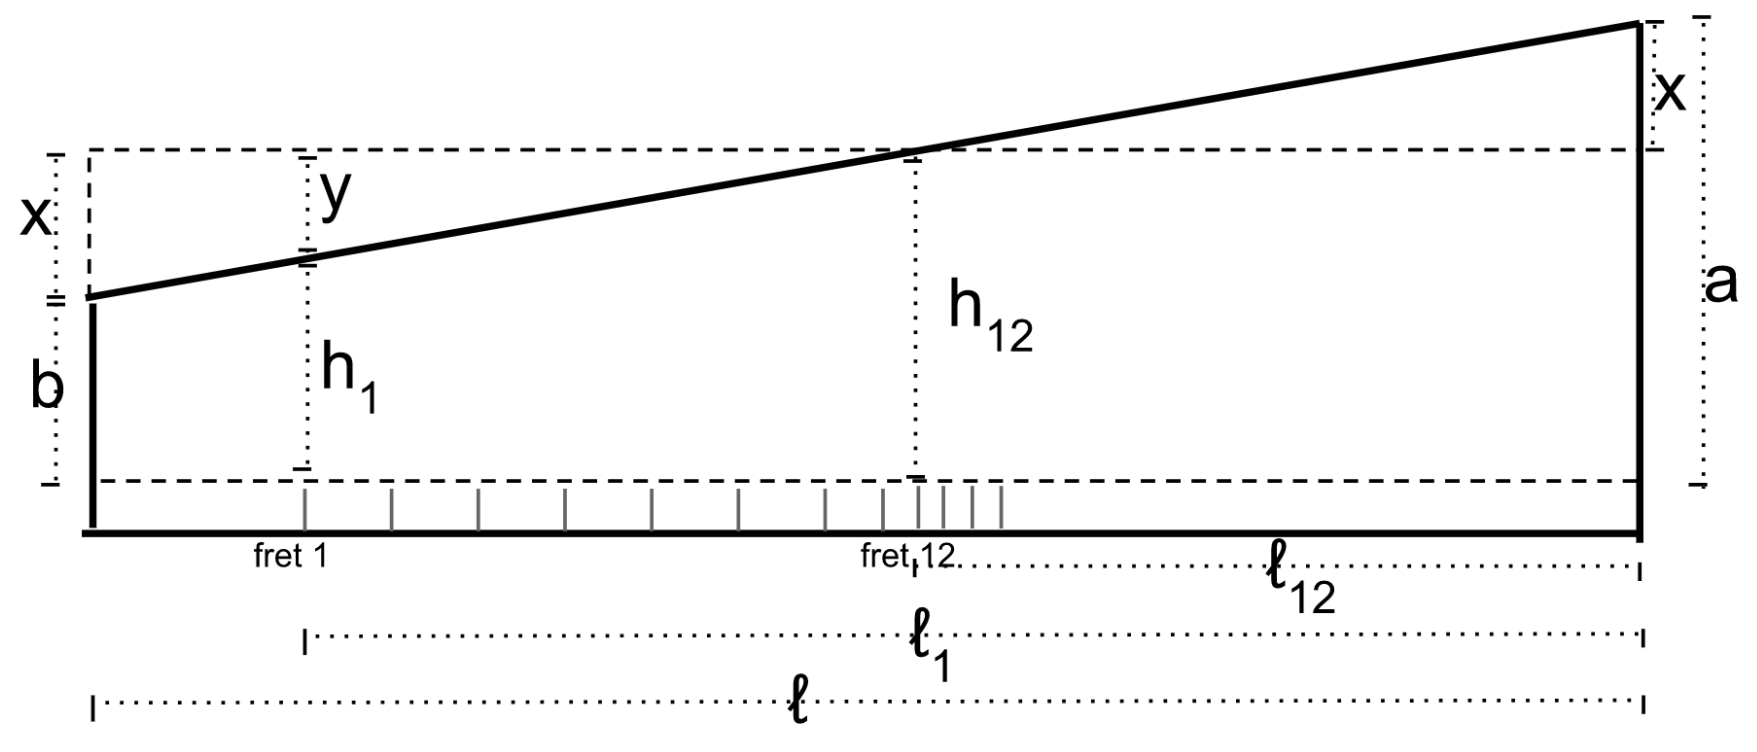
\includegraphics[width = \textwidth]{./ee/fig4.png}
    \caption{Diagram to calculate values of $a$ and $b$} \label{fig3}
\end{figure}
Since fret \nth{12} is exactly in the middle of $l$ ($l_{12} = \frac{l}{2} = \frac{0.648}{2} = 0.324$ m) we get:
\begin{align*}
    a &= h_{12} + x \\
    b &= h_{12} - x
\end{align*}
From the luthier formula (\ref{eqn2}):
\begin{align*}
    l_1 &= \frac{l}{2^{\frac{1}{12}}} \\
        &= \frac{0.648}{2^{\frac{1}{12}}} \\
        &= \SI{0.612}{\meter}
\end{align*}
and we also get the ratio in Figure \ref{fig3}
\begin{align*}
    \frac{x}{y} &= \frac{l-l_{12}}{l_1-l_{12}} \\
    x &= y\frac{l-l_{12}}{l_1-l_{12}} \\
    &= (h_{12}-h_1)\frac{l-l_{12}}{l_1-l_{12}} \\
    &= (1.78-0.406) \cdot 10^{-3} \cdot \frac{0.648-0.324}{0.612-0.324} \\
    &= \SI{1.55e-3}{\meter}
\end{align*}
Therefore
\begin{align*}
    a &= 1.78 + 1.55 = \SI{3.33e-3}{\meter} \\
    b &= 1.78 - 1.55 = \SI{1.30e-4}{\meter}
\end{align*}